\chapter{The benefits of prefetching for large-scale cloud-based neuroimaging
analysis workflows}~\label{chp:rp}



Valerie Hayot-Sasson$^1$, Tristan Glatard$^1$, Ariel Rokem$^2$ \\
\begingroup \footnotesize $^1$Department of Computer Science and Software
Engineering, Concordia University, Montreal, Canada\\
$^2$ Department of Psychology and eScience Institute, University of Washington,
Seattle, Washington, USA\\
\endgroup
\vspace{5pt} \\
Presented at (in press): \\
\hspace*{10pt} \textit{2021 16th Workshop on Workflows in Support of Large-Scale
Science:} \url{arXiv:2108.10496}

\section{Abstract}
%%edited
To support the growing demands of neuroscience applications, researchers are
transitioning to cloud computing for its scalable, robust and elastic
infrastructure. Nevertheless, large datasets residing in object stores may
result in significant data transfer overheads during workflow execution.
Prefetching, a method to mitigate the cost of reading in mixed workloads, masks
data transfer costs within processing time of prior tasks. We present an
implementation of ``Rolling Prefetch", a Python library that implements a
particular form of prefetching from AWS S3 object store, and we quantify its
benefits.

Rolling Prefetch extends \sfs, a Python library exposing AWS S3 functionality
via a file object, to add prefetch capabilities. In measured analysis
performance of a 500~GB brain connectivity dataset stored on S3, we found that
prefetching provides significant speed-ups of up to 1.86$\times$, even in
applications consisting entirely of data loading. The observed speed-up values
are consistent with our theoretical analysis. Our results demonstrate the
usefulness of prefetching for scientific data processing on cloud
infrastructures and provide an implementation applicable to various application
domains.


%%%%%%%%%%%%%%%% original

    % With the increase in dataset size and computing requirements of
    % neuroimaging workflows, researchers have transitioned to cloud
    % environments to provide the necessary infrastructure to enable the
    % research. Since compute-local storage on the cloud can be rather costly,
    % large datasets are placed on slower, but scalable, cloud storage
    % instances, resulting in non-negligible performance penalties when
    % accessing the data during workflow execution. A popular method for
    % mitigating the cost of data accesses is through prefetching. In
    % prefetching, the data is transferred fast storage in anticipation of a
    % task access, masking slow storage latency and bandwidth within task
    % scheduling and compute time.
    
    % In this paper, we investigate the benefit of prefetching on a neuroimaging
    % use case running on a t2-xlarge Amazon EC2 instance operating on an 500~GB
    % tractography dataset stored on Amazon S3. To achieve this, we designed a
    % model to describe the anticipated performance trends, developed a Python
    % library based on S3Fs to prefetch the data and compared its performance
    % with S3Fs as its baseline. Overall, it was found that prefetching the data
    % provided a significant speedup when large amounts of data needed to
    % processed by a task and when there were many parallel tasks accessing the
    % dataset.
 
 %%%%%%%%%%%%%%%%%%%%%
  %Neuroimaging deals with massive amounts of data. One way to deal with that is
  %to move to cloud computing. One of the persistent bottlenecks in %data
  %analysis in these environments is that you have to wait for data to arrive at
  %the CPU to be able to start analyzing it. Here, we devise a %way to prefetch
  %data that will be needed in the future, while other work is happening.

\section{Introduction}


% Cloud service providers, such as Amazon Web Services (\aws)~\cite{aws},
% Microsoft Azure~\cite{azure} and Google Cloud~\cite{gc}, give access to two
% main services: Compute services and Object Stores. Compute services typically
% consist of instances with a configured amount of RAM, vCPU and local storage.
% Costs associated with compute services increase with the number of resources
% and time required. Compared to object stores, compute-local storage can be
% very costly, particularly when storing large amounts of data for extended
% periods. Thus, users generally opt for scalable external object stores for
% their large data. This is despite the increased latency, which may vary
% depending on location of the storage and compute instance network. Examples of
% cloud object storage include Amazon's Simple Storage Service (S3), Azure's
% Blob Service, and Google Cloud Storage. 


Many fields of science are experiencing increases in the volume of datasets
available to researchers. Neuroscience in particular is experiencing a rapid
growth in data due to technical advances, scientific breakthroughs, and
sociological trends towards open data sharing. This increase in data is
providing the basis for new discoveries about brain structure and function, but
it also presents technical challenges. To deal with the deluge of available
data, neuroscientists are increasingly adopting cloud platforms for data storage
and processing. However, inefficient use of cloud services can lead to
needlessly longer processing time and cost. We aim to investigate methods to
reduce the impact of data transfers for neuroimaging workflows on cloud
services.

Data prefetching is a well-established technique for the reduction of data
access-related costs~\cite{callahan1991software, mowry1992design,
klaiber1991architecture}. Traditionally, prefetching was used to reduce memory
latency, as memory accesses were significantly slower than CPU processing.
However, since the rise of Big Data, prefetching has also been shown to be
beneficial to the processing of large datasets located on remote
storage~\cite{yildiz2018improving}. During the execution of an application, data
required for future tasks are copied from the remote storage device to
compute-local storage, such that when the application requires the data, it can
read it from local storage.

A recent example of the effectiveness of prefetching on the cloud is
Netco~\cite{jalaparti2018netco}, a prefetching extension integrated into the
Hadoop Distributed File System (HDFS). Future data is prefetched based on two
measures: 1) size of the data to be processed and 2) task deadline.  Netco
demonstrated superior performance compared to other file systems, which
importantly motivates our study. However, it remains tightly bound to HDFS while
cloud applications generally use different file systems. A more versatile
solution is needed that would broadly apply to cloud data analysis and storage.

The present study focuses on neuroscience data that describe long-range
connections between different parts of the human brain, a central research topic
in contemporary neuroscience~\cite{bassett_network_2017}. The three-dimensional
trajectory of the major neural pathways, composed of millions of neuronal axons,
are inferred from measurements of diffusion MRI and processed using
computational tractography algorithms. These algorithms generate ``streamlines":
3D curves that approximate the trajectories of the major pathways. A single
human brain measurement may contain several millions of these streamlines, with
their coordinates assessed at sub-millimeter resolution. Subsequent analyses of
these streamlines usually access streamlines sequentially and entirely within
the files in which they are stored. Such an access pattern creates an excellent
opportunity for prefetching.


This paper investigates the benefits of prefetching for cloud-based processing
of neuroscience streamlines. Through both theoretical analysis and
experimentation, we characterize the speed-up provided by prefetching compared
to sequential data transfers for neuroscience data processing deployed on the
Amazon Web Services cloud. More specifically, this paper makes the following
contributions: 
\begin{itemize}
    \item Formalization and performance analysis of a ``rolling prefetch" data
    scheme for cloud-based applications;
    \item Implementation based on the S3Fs Python library to access data on
    Amazon S3;
    \item Experimental evaluation in the Amazon cloud with a 500-GB dataset of
    streamlines derived from dMRI data.
\end{itemize}
% This is due to technical and scientific breakthroughs, enabling improved
% measurements that are providing more detailed views of the brain. But also
% thanks to sociotechnical trends that are  promoting increase sharing of
% neuroscientific data. For example, human brain imaging datasets are rapidly
% increasing in size. While many neuroimaging studies ranged from 10 - 100~GBs
% in size, newer datasets such as the BigBrain~\cite{amunts2013bigbrain}, UK
% Biobank~\cite{sudlow2015uk} and the Human Connectome Project
% (HCP)~\cite{van2013wu} are expected to reach up to Petabytes of data. Cloud
% platforms are commonly used to store this data in publicly-accessible object
% stores, as is the case for instance for \hcp data.



% \subsection{Cloud Infrastructure} The cloud gives users access various types
% of self-maintained services and hardware. This is a particularly attractive
% model to scientific groups who would not otherwise have the expertise nor the
% funds to maintain such infrastructure. Furthermore, the amount of
% infrastructure is vast, supporting many users without significant queuing time
% in attaining the resources. Unlike High Performance Computing (HPC) clusters
% which may also provide access to various self-maintained hardware, users using
% the cloud as an Infrastructure as a Service (IaaS), can install whatever
% software is required on there.


\section{Materials and Methods}

Our implementation of prefetching, known as Rolling Prefetch, is a Python
library implemented as a layer on top of \sfs. The code is available under the
MIT license at \url{https://github.com/ValHayot/rollingprefetch}. \sfs is a
Python library, based on FSSpec, for interacting with directories and files
located on Amazon S3. To offset the cost of latency on S3, \sfs leverages the
on-demand caching mechanisms provided by FSSpec.

Unlike \sfs which has distinct data transfer and compute phases, prefetched data
transfers happen concurrently with compute (Figure~\ref{fig:rp:prefetch}). In both
cases, data is transferred from cloud storage in blocks of configurable size.
While local I/O overheads occur during prefetch, the resulting overhead is in
general minimal since memory disks are expected to be used for this purpose.
Most importantly, prefetching requires knowledge of the application's data
access pattern, such that transfers can be correctly anticipated. In our case,
we assume that data is read sequentially, as is commonly the case with
tractography data.

Since Rolling Prefetch is implemented as a layer atop \sfs, it can easily
replace an existing call to S3Fs by calling \texttt{S3PrefetchFileSystem}
instead of \texttt{S3FileSystem}.

\begin{figure}
\begin{center}
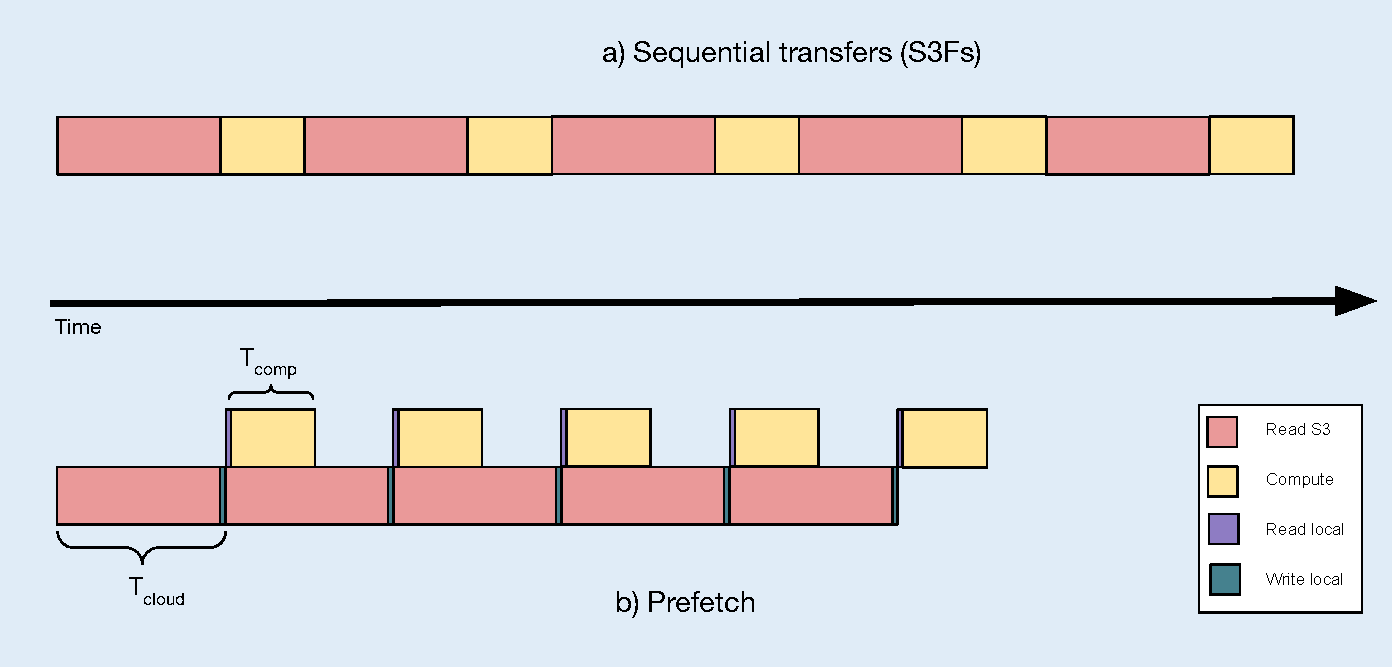
\includegraphics[width=\columnwidth]{figures/rp/prefetch_diagram.pdf}
\end{center}
\caption{Prefetching vs sequential transfers (\sfs)}
%https://docs.google.com/drawings/d/1MV5dIdLyBrM_HJX-0jOsIKf90UD8wXE_G5Cnmd-mY-A/edit
\label{fig:rp:prefetch}
\end{figure}

\subsection{Algorithm}


% These caching mechanisms include MMapCache, ReadAheadCache, BlockCache,
% BytesCache and AllBytes. AllBytes attempts to cache the entire file contents
% into memory upon data access. MMapCache creates a memory-mapped temporary file
% which is populated in units of blocks, based on the configurable
% \texttt{block\_size} parameter, as data is requested. For small sequential
% reads, the ReadAheadCache can be used to load data in blocks at a time. The
% BytesCache is similar to the ReadAheadCache except it improves the efficiency
% of semi-random reads by also maintaining parts of the previous cached block in
% memory. BlockCache differs from the others in that it implements a least
% recently used (LRU) cache of max number of blocks. When memory is filled, the
% least recently used block is evicted and the next one is read. By default,
% \sfs uses the BytesCache with a block size of 5~MB.

Rolling Prefetch combines prefetching with data eviction. By evicting processed
data, it ensures a reduced footprint on the local storage leveraged as cache
(e.g. tmpfs, SSD, HDD). Rolling Prefetch consists of three threads: (1) the
reading thread loads data blocks from local storage and marks them for eviction,
(2) the prefetching thread transfers data blocks from cloud storage to local
storage, and (3) the eviction threads deletes the blocks that have been marked
for eviction.
% \valerie{cut read alg below} \begin{algorithm} \SetAlgoLined
% \SetKwInOut{Input}{Input} \SetKwInOut{Output}{Output} \Input{$start$ the start
% position of the read;\\
%     $end$ the end position of the read;\\} \Output{$output$ the file contents
%     located between $start$ and $end$}
    
%     $not\_local \gets True$\;
    
%     $read\_length \gets 0$ $total\_read \gets end - start$
    
%     \While{$total\_read > read\_length$}{ \While{$not\_local$}{ $block,
%         not\_local \gets check\_local(start)$\;
%         }
        
%         $curr\_end \gets max(block.end, end)$\; $output \gets
%         block.read(start, curr\_end)$\;
        
%         \If{$block.end < end$}{ $start \gets curr\_end$\;
%             $flag\_for\_deletion(block)$\;
%         }
        
%     }
    
% \caption{Read}\label{alg:read} \end{algorithm}

\subsubsection{Reading}

The reading thread is triggered by the application to read data directly from
cache or to wait until it is prefetched, if not found in the cache.
%(Algorithm~\ref{alg:read}).
By waiting for the data to be cached, we ensure that performance is comparable
to \sfs in the worst case scenario. Furthermore, as all data reads are considered
to be sequential, if the current block is not in memory then it is the current
block being prefetched. Whenever a prefetched block has been read fully, it is
up to the read function to flag it for deletion.
% This process involves renaming the file to contain a ``.todelete'' extension.
% Using this extension, the eviction thread can determine which files need to be
% deleted.

\subsubsection{Prefetching}

Throughout the lifetime of the application, the prefetching thread continuously
requests blocks from cloud storage, so long as there remain blocks that have not
been prefetched (Algorithm~\ref{alg:rp:prefetch}). Each block will be written to an
appropriate cache location while not exceeding user-defined space limits.

Initially, the \texttt{used} variable for all cache locations is set to zero and
the \texttt{file\_index} variable is set to point to the first file index in the
sequential ordering. The algorithm then enters a while loop whose termination is
dictated by the main program.
% (i.e., if the file object is still open, fetch, otherwise, terminate thread).
If all files have been prefetched, the prefetching threads terminates regardless
of the status of the main thread. Within the loop, the algorithm iterates
between all available cache locations in priority order. The amount of available
storage space remaining is computed, and if it is insufficient to write the next
block, the algorithm iterates through the file list $total\_files$
($verify\_used()$) and queries the file system to determine which blocks have
been evicted. Based on how many blocks have been removed, we can update the
amount of used space, and by extension, the amount of available space. Should
sufficient space be released, the next block is fetched from cloud storage and
is written to local storage. If there is insufficient space, the next local
storage location is tried.

%%mention in discussion the risk of an infinite loop if insufficient cache
% location storage space is provided. maybe need for timeout? -- will not
% mention!

\begin{algorithm2e}
\SetAlgoLined \SetKwInOut{Input}{Input} \Input{ $fetch$ a shared variable
    indicating whether the main thread has terminated or not\\
    $total\_files$ the list of all the files to prefetch;\\
    $cache\_location$ list of paths to cache locations;\\
    $total$ total space available on prefetch cache;\\
    $total\_size$ cumulative sum of all prefetched files;\\
    $blocksize$ size of a block\\}
    
$used \gets 0$\; $file\_index \gets 0$\; \While{$fetch$}{
\ForEach{$cache\_location$}{ $available \leftarrow total - used$\; \If{
$available < blocksize$}{ $available \gets verify\_used()$\; } \If{ $available
\geq blocksize$}{ $fetch\_next\_block()$\; $used \leftarrow used + blocksize$\;
} } \If{$total\_size \leq offset$ or $file\_index + 1 < total\_files$}{
$file\_index \gets file\_index + 1$\; $total\_size \gets
sizeof(total\_files[file\_index])$\; } \ElseIf{$total\_size \leq offset$}{
break; } } \caption{Prefetching}\label{alg:rp:prefetch}
\end{algorithm2e}



\subsubsection{Eviction}

Similar to prefetching, the eviction thread only terminates when the main thread
has completed processing. %(Algorithm~\ref{alg:eviction}).
% However, there is no mechanism for it to break prior to the main thread
% indicating termination. This is because we assume that the file object will be
% closed when all data has been read.
To avoid additional costs caused by continuously querying the filesystem to
determine which files can be evicted, we determine the names of all the blocks
that should be evicted ($get\_all\_blocks$), and verify whether they exist in
the file system at time of removal. We then update the list to ensure that we do
not attempt to remove this file more than once. Between each loop, we sleep for
5 seconds to ensure that sufficient time has elapsed between evictions.

The eviction thread ensures deletion of all remaining files prior to
terminating.


% \valerie{cut eviction alg below} \begin{algorithm} \SetAlgoLined
% \SetKwInOut{Input}{Input} \Input{$fetch$ a shared variable indicating whether
% the main thread has terminated or not;\\
%     $total\_files$ a list files to prefetch;\\
%     $cache\_location$ a list of paths to cache locations;\\
%     $file\_sizes$ a list containing the size of each file;\\
%     $blocksize$ size of a block\\}
    
%     $all\_blocks \gets get\_all\_blocks()$\;
    
%     \While{fetch}{ \ForEach{$block$ in $all\_blocks$}{ \ForEach{$dir$ in
%         $cache\_location$}{ $removed \gets remove(block)$\;
                
%                 \If{$removed$}{ $update\_list(all\_blocks, block)$\; break\;
%                 }
                
%             }
%         }
%         $sleep 5$\;
%     }
%     $remove\_remaining(all\_blocks)$

% \caption{Eviction}\label{alg:eviction} \end{algorithm}

\subsection{Performance analysis}

We consider the cost of processing a file using sequential transfers (\sfs) to
be the sum of three components (Equation~\ref{eq:rp:s3fs}): 1) latency-associated
costs, 2) bandwidth-associated costs and 3) application compute time. The cost
of latency is experienced every time a chunk of data is requested from cloud
storage. That is, if we read a full file in a single call to cloud storage, we
will only pay for latency once. If we issue multiple calls to obtain file data
on cloud storage, we will pay latency for each call. In contrast, bandwidth is
not affected by the number of calls. Whether we request all the data at once or
in chunks, bandwidth remains fixed, and time to transfer the data is the
quotient between the total amount of data transferred and the bandwidth. Compute
time is assumed to be proportional to data size, as is frequently the case in
neuroimaging.

    \begin{equation}
T_{\mathrm{seq}} = n_{b}l_c + \frac{f}{b_{cr}} +  cf,
\label{eq:rp:s3fs}
\end{equation}
where $n_{b}$ is the number of data blocks, $f$ is the total size of the file to
transfer, $l_c$ is the cloud latency, $b_{cr}$ is the cloud read bandwidth, and
$c$ is the compute time per byte consumed.

Rolling Prefetch contrasts Equation~\ref{eq:rp:s3fs} in that the compute and data
transfer times mask one another (Equation~\ref{eq:rp:prefetch}). However, Rolling
Prefetch has a slightly higher performance penalty than that of sequential
transfers when there is no compute, due to reading and writing the data to local
storage. Furthermore, we must consider the initial read from cloud storage,
where no compute can occur concurrently, and the last compute, where no data
transfer can occur concurrently.

\begin{equation}
T_{\mathrm{pf}} = T_{\mathrm{cloud}} + (n_b-1)\max\left(T_{\mathrm{cloud}}, T_{\mathrm{comp}}\right) + T_{\mathrm{comp}} \label{eq:rp:prefetch}
\end{equation}
where $T_{\mathrm{cloud}}$ is the time to download a block from the cloud and
write it to local storage, and $T_{\mathrm{comp}}$ is the time to read a block
from local storage and process it:
\begin{eqnarray*}
T_{\mathrm{cloud}} &=& \overbrace{l_{c} + \frac{f}{b_{cr}n_{b}}}^{\mathrm{cloud\
read}} + \overbrace{l_{l} + \frac{f}{b_{lw}n_{b}}}^{\mathrm{local\ write}}, \\
T_{\mathrm{comp}} &=& \underbrace{l_l+\frac{f}{b_{lr}n_b}}_{\mathrm{local\
read}} + \underbrace{\frac{cf}{n_b}}_{\mathrm{compute}},
\end{eqnarray*}
where $l_l$ is the latency of local storage, $b_{lw}$ is the write bandwidth to
local storage, and $b_{lr}$ is the read bandwidth to local storage.

This simple model provides several insights. First, if we neglect local
transfers ($l_l$=0, $b_{lw}$=$b_{lr}$=+$\infty$), a reasonable assumption when
local storage is in-memory, then we have:
\begin{equation*}
T_{\mathrm{seq}} = T_{\mathrm{pf}} + (n_b-1)\min\left(T_{\mathrm{cloud}},T_{\mathrm{comp}}\right),
\end{equation*}
and therefore the speed-up provided by Rolling Prefetch compared to sequential
transfers is:
\begin{equation}
S=\frac{T_{\mathrm{seq}}}{T_{\mathrm{pf}}}=1+(n_b-1)\frac{\min\left(T_{\mathrm{cloud}},T_{\mathrm{comp}}\right)}{T_{\mathrm{pf}}} < 2 
\label{eq:rp:speed-up}
\end{equation}
Rolling Prefetch is therefore expected to provide a speed-up of at most 2x. This
upper bound is approached when $T_{\mathrm{cloud}} \approx T_{\mathrm{comp}}$,
which requires that cloud transfer and compute times are of similar magnitude.

In sequential transfers, using a single block ($n_b=1$) leads to the shortest
transfer time. In practice, block size is of course constrained by available
memory. In contrast, with Rolling Prefetch, an optimal block size $\hat n_b$
exists under the reasonable assumption that $l_l \ll l_c$:
\begin{equation}
    \hat n_b = \sqrt{\frac{cf}{l_c}}
\end{equation}
It suggests that on a given cloud infrastructure, the number of blocks should
increase when the application compute time or the total data size increases.

Finally, as the number of blocks increases, $T_{\mathrm{seq}}$ and
$T_{\mathrm{pf}}$ become equivalent to $n_bl_c$ and $n_b(l_c+l_l)$,
respectively, resulting in parallel asymptote lines.

%\tristan{Processing time should be explained when you explain the problem in
% intro. The real question in this paper is whether opening (and processing)
% tractography files involves enough data transfers AND compute time for
% prefetching to be useful. If one is negligible compared to the other, speed-up
% will be negligible too.} \ariel{Added a suggested subsection describing the
% dataset} \valerie{cut entire implementation subsection} \tristan{I moved the
% description of S3FS here, you could summarize the paragraphs on your
% implementation into 1} \subsection{Implementation}

% Rolling prefetch is a Python library implemented as a layer on top of \sfs.
% \sfs is a Python library, based on FSSpec, for interacting with directories
% and files located on Amazon S3. To offset the cost of latency on S3, \sfs
% leverages the on-demand caching mechanisms provided by FSSpec. These caching
% mechanisms include MMapCache, ReadAheadCache, BlockCache, BytesCache and
% AllBytes. AllBytes attempts to cache the entire file contents into memory upon
% data access. MMapCache creates a memory-mapped temporary file which is
% populated in units of blocks, based on the configurable \texttt{block\_size}
% parameter, as data is requested. For small sequential reads, the
% ReadAheadCache can be used to load data in blocks at a time. The BytesCache is
% similar to the ReadAheadCache except it improves the efficiency of semi-random
% reads by also maintaining parts of the previous cached block in memory.
% BlockCache differs from the others in that it implements a least recently used
% (LRU) cache of max number of blocks. When memory is filled, the least recently
% used block is evicted and the next one is read. By default, \sfs uses the
% BytesCache with a block size of 5~MB.

% \subsection{Implementation details}

% Inheriting functionality from \sfs permitted us to focus on prefetching rather
% that the logic of communicating directly with the S3 interface. However, we
% have modified some of the S3Fs functions, settings and functionality. 

% \begin{sloppypar} The implementation can be split up into two classes:
% \texttt{S3PrefetchFileSystem} and \texttt{S3PrefetchFile}.
% \texttt{S3PrefetchFileSystem} inherits from \sfs' \texttt{S3FileSystem}, and
% is nearly identical to the S3FileSystem class, with the exception that it
% overrides S3FileSystem's call to \texttt{open} to create and return an
% \texttt{S3PrefetchFile} object. \end{sloppypar}

% % Aside from reimplementing the \texttt{read} function, S3File is responsible
% for starting and stopping the prefetch and evictions threads. Both the
% prefetch and eviction threads are instatiated in the constructor of an
% S3PrefetchFile. % The threads are then terminated via the status % of a shared
% object (i.e. $self.fetch$) between the threads. % The most important
% difference between \texttt{S3File} and \texttt{S3PrefetchFile} is that we have
% disabled \sfs caching in our library, since it is embedded in prefetching. 

% Since it is common for large files to be broken down into datasets of smaller
% files, we wanted the ability to leverage prefetching in this case. As a
% result, a call to open accepts a list of file paths rather than just a single
% path. In the case where there needs to be a header, the first file in the
% provided list must point to the header region. If all the other files contain
% a header that needs to be skipped, there is a parameter, known as
% \texttt{header\_bytes} that can be passed to \texttt{open} to specify the size
% of the header to skip in subsequent files. Currently, it is not possible to
% prefetch unrelated files.

% % \begin{sloppypar} % The library fixes the open mode to be ``read bytes'', as
% \texttt{S3PrefetchFile} is only intended to read files, and currently only
% functions with binary files. To be able to write or append to files, the
% \texttt{open} of the parent class of \texttt{S3PrefetchFileSystem} % will need
% to be used. % \end{sloppypar}

% Prefetching should be enabled to write to any available local filesystem. As a
% result, we have added the \texttt{prefetch\_storage} parameter to the
% initialization of an \texttt{S3PrefetchFile}. This parameter allows users to
% specify the desired caching locations and the amount of available space to use
% at each location. The cache directories are listed in terms of descending
% priority. That is, the first location should point a location on the fastest
% available local storage, e.g., tmpfs.

\subsection{Data}

To demonstrate the utility of Rolling Prefetch in neuroimaging, we analyzed data
derived from a dMRI experiment conducted in a single subject. These data are
special, in that a  Super-Resolution Hybrid Diffusion Imaging (HYDI) method was
used to achieve an effective spatial resolution of 0.625 mm$^3$, much higher
than the typical $\sim$2 mm$^3$ commonly used. The details of the HYDI method
and parameters of data acquisition were previously described
\cite{Elsaid2019-ez}. The source MRI data were 14.94 GB. The data were processed
using a probabilistic tractography algorithm \cite{Berman2008-xg}, implemented
as part of DIPY \cite{Garyfallidis2014-el} and accelerated using CUDA to work on
GPU \cite{rokem2021gpu}. This  generated $\sim$498 GB of streamline data.
Tractography streamlines are usually stored in the neuroscience-specific
\texttt{.trk} file format. In this case, streamlines were sharded into 464
\texttt{.trk} files stored in an S3 bucket using the high-availability Standard
storage class. 

% \tristan{I moved the nibabel text here, it could be summarized in 1 paragraph}
% \ariel{ I revised the nibabel section into one paragraph. Below in comments is
% the original as I found it:}
 Each \texttt{.trk} file consists of a 1,000-byte header and a body of
variable length consisting of a series of streamlines. Each streamline section
contains \SI{4}{\byte} that denote the number of points in the streamline,
followed by a series of floating point values detailing each coordinate and ends
with a series of values representing properties of the streamline. We used
NiBabel, a Python library that reads and writes  neuroscience-specific data
formats, to read these files. For \texttt{.trk} files, NiBabel can return
individual data points via a generator. This is known as ``lazy loading'' and
can be turned on or off prior to reading the file. As a result of the data
representation format in \texttt{.trk} files, NiBabel reads may incur
significant overhead: because it issues a total of three read calls for each
streamline in the file.
% , some of which can be very small, depending on the streamline.
In addition, an affine transform is stored together with the data, and used to
bring coordinates from different measurements into register. For example, when
NiBabel reads \texttt{.trk} files it automatically applies an affine
transformation to the coordinates of each streamline stored in the file. This
means that some amount of compute is always executed when data is read from
file.

% As in many other research fields, neuroscience data is usually stored in
% field-specific file formats. For example, MR images are often stored in the
% Neuroimaging Informatics Technology Initiative (NIfTI) file format, with the
% \texttt{.nii}  extension. Streamlines from computational tractography are
% often stored in a file format based on the Trackvis software, with the
% \texttt{.trk} extension. Nibabel is a Python library that implements reading
% and writing of many neuroscience-specific data formats. It is highly used in
% Python-based analysis projects of neuroimaging data. For files that exceed
% available memory, it provides the ability to MemoryMap them, it the case of
% randomly accessed files, or it returns individual data points via a generator,
% for sequentially accessed files. This is known as ``lazy loading'' and can be
% turned on or off prior to reading the file. In the case of \texttt{.trk} files
% representing streamlines, as they are sequentially read, Nibabel uses a
% generator to return streamlines.

% As a result of the data representation format in \texttt{.trk} files, Nibabel
% may incur significant overheads when reading them. Each \texttt{.trk} file is
% comprised of a 1000 byte header and a body of variable length consisting of a
% series of streamlines. Each streamline contains \SI{4}{\byte} that denote the
% number of points in the track, followed by a series of floating point values
% detailing each track point and ends with a series of values representing the
% properties of the track. This means that for each existing streamline, Nibabel
% issues a total of three read calls, some of which can be very small, depending
% on the streamline.

% One of the challenges of analyzing volumetric data from neuroimaging is that
% the origin, voxel size and orientation of the acquisition volume can vary
% between different acquisitions (e.g., different MRI contrasts). To correspond
% the data from these different acquisitions, affine transforms are stored
% together with the data, and the transforms can be applied to the coordinates
% of different data to bring them into register. For example, when Nibabel reads
% \texttt{.trk} files it automatically applies an affine transformation to the
% coordinates of each streamline stored in the file. This means that some amount
% of compute is always executed when data is read from file.

\subsection{Experiments}
To evaluate the performance Rolling Prefetch, we conducted four experiments: 1)
varying the number of files; 2) varying the blocksize; 3) parallel processing of
files;  and 4) neuroimaging use-cases. For experiments 1-3, the pipeline
consisted of reading the file with NiBabel. As NiBabel performs a minimal amount
of computing, Rolling Prefetch is believed to have an effect even here.
Additional compute required by real analysis should only increase the benefit of
using prefetching.
% For all experiments we are using tractography files belonging to the HYDI
% dataset stored on S3.

\subsubsection{Varying the number of files}\label{exp:rp:files}

We vary the number of \texttt{.trk} files read to determine when Rolling
Prefetch will be favourable relative to \sfs. We expect that for small amount of
data, there should be no significant discernible difference between \sfs and
Rolling Prefetch. This is because compute time is expected to be minimal and the
blocksize large compared to the total dataset size. In other words, there will
be less opportunities to prefetch data with very small datasets, unless the
block size is proportionally smaller, in which case latency will be penalizing
both reads from \sfs and Rolling Prefetch, extending processing time. With
larger files, there will be more computation occurring during the reads, and
therefore, more opportunities to mask the data transfers within the compute.

We benchmarked the time it took to lazily read 1, 5, 10, 15, 20 and 25 files and
extract the streamlines in NiBabel. The total data size for each of the file
increments are 1.1, 5.8, 11.9, 18.0, 24.2 and \SI{31.2}{\gibi\byte},
respectively. The blocksize was set to \SI{64}{\mebi\byte} and the prefetch
storage was located on \texttt{tmpfs} with a limit of \SI{2}{\gibi\byte} of
storage space. We performed 10 repetitions.

\subsubsection{Varying the blocksize}\label{exp:blocksize} In this experiment,
we aimed to quantify the effect of the number of blocks ($n_b$) on Rolling
Prefetch and \sfs. According to our performance analysis, we expect that \sfs
will reach its best performance with a single block, and that the runtime will
linearly increase with $n_b$ from that point on. For Rolling Prefetch, we expect
the runtime to decrease to a minimum, and then increase linearly with $n_b$.


Block sizes of 8, 16, 32, 64, 128, 256, 512, 1024, and \SI{2048}{\mebi\byte}
were used to load the files into NiBabel and extract the streamlines.
% We suspect that \SI{8}{\mebi\byte} may be too small to have many computes
% spanning more than a single block, however, it will occur at a higher
% frequency then with larger blocks.
We use the largest-sized block (\SI{2048}{\mebi\byte}) to determine the overhead
of using the Rolling Prefetch algorithm, as no file in the HYDI dataset is
larger than \SI{1.7}{\gibi\byte}, and therefore, there are no opportunities to
prefetch.

Five files pertaining to the HYDI dataset were used to generate the results.
These files ranged from \SI{793}{\mebi\byte} to \SI{1.5}{\gibi\byte} in size
each. Since only Rolling Prefetch is capable of treating a list of files as a
single file, a new NiBabel object needed to be created for each file in the case
of \sfs.

The experiment was executed on both \sfs and Rolling Prefetch for each block and
repeated 10 times. Prefetched storage was set to be \texttt{tmpfs} and
configured to have \SI{2}{\gibi\byte} of available space such that the largest
block size could fit in prefetch storage.

\subsubsection{Parallel processing}\label{exp:rp:parallel}

Since perceived throughput may be affected by the number of threads used, we
aimed to determine if the performance difference between \sfs and Rolling
Prefetch remains proportional to the amount of data being processed per thread. 

If throughput is reduced by the number of active threads, it is expected that
the cost of data transfers will outweigh the cost of computing, such that the
difference between \sfs and Rolling Prefetch will be very small. Furthermore,
since S3 is a scalable distributed file system and local storage may not be (or
may be more limited in terms of scalability), local storage throughput is
expected to be reduced significantly with the addition of multiple threads. 
% Should this be the case, the overheads specific to prefetching will become
% very costly.

We used a total of four parallel processes to evaluate the effects of parallel
processing. We increased the number of files per thread between each condition
from 1-20, with the last condition loading a total of \SI{108}{\gibi\byte} into
NiBabel. The blocksize was set to \SI{64}{\mebi\byte} and we set the prefetch
storage location to be on \texttt{tmpfs}, with a limit of \SI{1}{\gibi\byte} of
storage per process. 10 repetitions were performed.

\subsubsection{Neuroimaging use cases}\label{exp:rp:4} Our previous experiments
evaluate the value of Rolling Prefetch when the application performs the most
basic and necessary action: converting the data from binary to array
representation.
% Although it is unusual for applications to load the data without performing
% any additional processing of any kind, this will give us an idea of the lower
% bound of speedups .
We expect that the benefits of Rolling Prefetch can be maximized with an
increased compute time, due to greater opportunities to prefetch data during
compute. However, we also expect that there is a peak ratio between data
transfer time and compute time (data-to-compute ratio), where the benefits of
Rolling Prefetch will be highest. If compute time is significantly greater than
data transfer, regardless of all the time saved by prefetching data, the total
runtime will predominantly be compute. This motivates further profiling to
determine how to shard large datasets, like the HYDI dataset, such that the
benefits of Rolling Prefetch can be maximized.


Since the benefits of Rolling Prefetch may vary according to the ratio between
data transfer and compute time, we have selected two use cases with varying
computation times: 1) histogram distribution of streamline lengths; and 2)
bundle recognition.

The distribution of streamline lengths is used in order to assess the
performance of tractography algorithms. It may also aid in determining if the
files are good candidates for compression. The histogram computation consists of
loading each streamline within the dataset lazily, gathering the lengths of each
individual streamline and generating a histogram of 20 bins from their lengths.
% Unlike the segmentation application, this application is data-intensive. 

The human brain is composed of multiple different functional regions, and these
regions are connected through major anatomical pathways. One of the first steps
in the analysis of streamline data from human brain dMRI data is to classify the
streamlines according to their three-dimensional trajectory into these different
pathways. This is referred to as ``bundle
recognition"~\cite{garyfallidis2018recognition}. To demonstrate the benefits of
Rolling Prefetch in this use-case, we ran a software pipeline that determines
whether streamlines within the tractography file belong to either of two
different bundles (the corticospinal tract, CST and the arcuate fasciculus,
ARC), or to neither \cite{Kruper2021-bo}. Currently, the pipeline loads the data
all at once (i.e. no lazy loading) and then performs the bundle recognition
task. Thus, it is not possible to read only fragments of a large file which does
not fit in memory, in this case, and as a consequence of the separation of data
loading and processing, there will be no opportunities to keep the prefetched
data transfers masked within compute operations. 

We chose not to modify the pipeline in order to determine what is the speedup
provided by Rolling Prefetch without additional optimization, and in order to be
able to speculate on the possible benefits of adapting existing pipelines to
support larger-than-memory files and allowing reads and computations to occur
together.

Varying parameters were used for the bundle recognition and histogram
application. For instance, recognition was executed on two different compute
instances (c5.9xlarge and r5.4xlarge). The experiment executed on the c5.9xlarge
instance consisted of a \SI{1}{\gibi\byte} file with a \SI{64}{\mebi\byte}
blocksize, whereas the experiment executed on the r5.4xlarge instance used 10
files totaling \SI{12}{\gibi\byte} and was configured to use a
\SI{32}{\mebi\byte} blocksize. 

The histogram experiment was executed on a r5.4xlarge instance with a
\SI{1}{\gibi\byte} file from the HYDI dataset and used a \SI{32}{\mebi\byte}
blocksize.

We also considered the speedups obtained from bundle recognition in smaller
files. We split up the previous \SI{1}{\gibi\byte} file and split it up into 9
shards containing the same number of streamlines. File sizes ranged from
\SI{73}{\mebi\byte} to \SI{165}{\mebi\byte}. We compared the speedup provided by
Rolling Prefetch on a \SI{165}{\mebi\byte} shard to the processing of all 9
shards. These experiments were run exclusively on the r5.4xlarge instance with
10 repetitions.

% To compare the benefits of Rolling Prefetch with different data-to-compute
% ratios, we executed the histogram computation and the bundle recognition
% algorithm on an r5.4xlarge instance using the \SI{1}{\gibi\byte} file.
% Blocksize in both cases was fixed at \SI{32}{\mebi\byte}. 5 repetitions were
% performed.

In all cases, \SI{2}{\gibi\byte} of cache storage was allocated to Rolling
Prefetch.

\subsection{Infrastructure}

For the first three experiments, we used an Amazon EC2 t2.xlarge instance with 4
vCPUs and \SI{16}{\gibi\byte} of RAM with a maximum of \SI{7.8}{\gibi\byte} of
RAM of \texttt{tmpfs} space. The compute instance was configured to use Red Hat
Enterprise Linux 8.3 with kernel version 4.18.0. This instance was hosted in
availability zone \texttt{us-west-2a}. The experiments all used Python version
3.9.0 with version 0.5.2 of \sfs and NiBabel version 3.2.1.

The scientific applications required significantly more memory than available on
t2.xlarge instances. As a result, they were executed on a c5.9xlarge instance
and a r5.4xlarge configured identically to the t2.xlarge instance, but located
in the \texttt{us-west-2d} availability zone. c5.9xlarge instances consist of 64
vCPUs and have \SI{72}{\gibi\byte} of available memory, whereas the r5.4xlarge
instance consists of 16 vCPUs and \SI{128}{\gibi\byte} of available memory. 

The data used for all experiments originated from the HYDI tractography dataset
stored on the Amazon S3 object store. This dataset is broken down into 464 files
ranging from \SI{700}{\mebi\byte} to \SI{1.7}{\gibi\byte} each. This dataset was
also located in the \texttt{us-west-2} region.

To get an idea of the cost of data transfers, we measured the time it would take
to read data sequentially from S3 to the t2.xLarge instance. We varied the
filesize from \SI{1}{\kibi\byte} to \SI{4}{\gibi\byte} and measure the time it
took to read the files from a \texttt{us-west-2} S3 bucket and from
\texttt{tmpfs}. This method was favoured over more standard benchmarking
libraries to ensure the two file systems were benchmarked in the same way.
Results were then compared to benchmarking results produced by the
\href{https://github.com/dvassallo/s3-benchmark}{s3-benchmark} library to ensure
validity of our benchmarking method. The results can be seen in
Table~\ref{table:rp:benchmarks}.


%%tristan do i keep this if our model is just a theoretical eval? maybe it
%should be placed where the model % is instead?
\begin{table}
\caption{Measured latency and bandwidth obtained from reading files ranging from
\SI{1}{\kibi\byte} to \SI{4}{\gibi\byte} on a t2.xLarge instance reading from an
S3 bucket in the same region.}
\centering
\begin{tabular}{| c | c | c| }
\cline{2-3}
  \multicolumn{1}{c|}{}& S3 & memory \\ 
  \hline
 bandwidth (MB/s) & 91 & 2221 \\  
 latency (s) & 0.1 & $\num{1.6e-6}$ \\
 \hline
\end{tabular}
\label{table:rp:benchmarks}
\end{table}


\section{Results}
\subsection{Varying the file size}
As we increase the file size we observe that the disparity between \sfs and
Rolling Prefetch increases (Figure~\ref{fig:rp:filesize}), with Rolling Prefetch
significantly outpacing ($\sim$1.7$\times$ faster) \sfs at \SI{31.2}{\gibi\byte} (25
files). This is expected as per our theoretical evaluation. With a large amount
of blocks, the pipeline duration is determined by the maximum between the time
it takes to compute the data $T_{comp}$ and the time it takes to transfer the
data $T_{cloud}$. On the other hand, \sfs runtime is the sum of the time it
takes to transfer the data and the compute. In this case, the compute time is
large enough such that using Rolling Prefetch significantly reduces runtime with
large amounts of data.

As the size of the data decreases, the benefit of using Rolling Prefetch also
decreases. 
% This too is expected, as there is proportionally less compute occurring.
In this particular use case, S3 data transfer time is much larger than that of
compute time, thus the only time we can save is that of $T_{comp}$. $T_{comp}$
like ${T_{cloud}}$ is proportional to the number of blocks used, and thus the
amount of time saved increases with file size. In the worst case, Rolling
Prefetch performance equals that of \sfs.

\subsection{Varying the block size}%% some parts may be better suited for discussion

At a very large number of blocks, the performance of both \sfs and Rolling
Prefetch is degraded due to increased impacts of both S3 storage latency and, in
the case of Rolling Prefetch, local storage latency
(Figure~\ref{fig:rp:blocksize}).  \sfs starts to surpass the speed of Rolling
Prefetch, although not substantially (approx. 1.03$\times$) at 748 blocks.
Furthermore, while we read from S3 at certain blocksizes, the block size on
local storage is dictated by file system and kernel readahead size. In our
specific case, the data would be read from \texttt{tmpfs}, and thus we do not
see a significant added cost to Rolling Prefetch. It could be inferred that the
overhead of Rolling Prefetch may be more significant with many
blocks due to NiBabel's access patterns, which consist of many small reads.

Conversely, when decreasing the number of blocks we see an increase in
performance in both \sfs and Rolling Prefetch. This is because both benefit from
decreased latency to access data on S3, by making fewer read calls to it.
Rolling Prefetch is found to be faster than \sfs with a peak speedup of 1.24~X
at 187 blocks (i.e. \SI{32}{\mebi\byte} blocks). The speedup obtained from
Rolling Prefetch did not vary significantly between 24 and 187 blocks, averaging
at a speedup of approximately 1.2~X. Rolling Prefetch outpaces \sfs at less than
748 blocks as the cost of local latency has diminished sufficiently with the
larger blocks. As the blocksize increases, Rolling Prefetch is able to begin
masking S3 latency and bandwidth within its compute.
% The speedup being proportional to how many more blocks can be read within the
% computation.
\sfs and Rolling Prefetch performance converges again when the blocks reach a
certain size, placing more weight disk bandwidth than latency. \sfs exceeds the
performance of Rolling Prefetch at a single block, where no actual prefetching
can take place and we pay the cost of implementation overheads, such as writing
the data to local storage and reading it from local storage rather than directly
from memory.

Generally speaking, variations in blocksize did not lead to major speedups
between Rolling Prefetch and \sfs. Since the total files size and compute time
was fixed, there was a fixed upper bound to how many data transfers could be
masked by compute time. By minimizing the amount of latency through a reduction
in the number of blocks, the overall application time was shortened, in both
\sfs and Rolling Prefetch, and thus a larger percentage of the total runtime
could be masked by compute.

\subsection{Parallelized workloads}
% \tristan{This section refers to file numbers while figure is in GiB}
When we parallelize the reads up to four concurrent processes
(Figure~\ref{fig:rp:parallel}), we notice that the trends are still consistent
despite increased contention on local filesystems. This is likely due to the
fact that \texttt{tmpfs} speeds would remain sufficiently high even with the
increased contention caused by having at minimum 4 and potentially even up to 8
concurrent threads accessing the file system at the same time. We speculate that
the same pipeline running with data read from a single disk would have had worse
performance due to its lack of scalability.

The maximum speedup achieved, on average, during this experiment was
1.86$\times$ at 24.2~GiB. The average speedup was around 1.52$\times$
altogether, with the minimum average speedup being 1.37$\times$ at 80.6~GB. Due
to the high variability in results within both Rolling Prefetch and \sfs, we
expect that these speedup differences may be a result of bandwidth and latency
variability across runs. We do not expect that conditions are more favourable
for reading the data with four threads processing 24.2~GiB; since they are
processing the same amount of data concurrently, the overall speedup should be
constant.

\subsection{Neuroimaging use-cases}

The results obtained from our neuroimaging use cases indicate that, in all
cases, the use of Rolling Prefetch can speed up analyses
(Figure~\ref{fig:rp:speedup}). The extent of this speedup is, however, dependent on
a number of factors, such as instance type, application and number of shards.

The greatest observed speedup with Rolling Prefetch was found when executing the
bundle recognition application with a greater number of shards (1.64$\times$
faster). This result echoes what was observed in Figure~\ref{fig:rp:filesize} with
even a more compute-intensive application like bundle recognition. We do not,
however, observe a speedup with a single shard, as the size of the shard was so
small it did not incur many reads from S3.

Due to the compute-intensive nature of the bundle recognition pipeline, it comes
as no surprise that overall speedup in the unsharded case is minimal
(1.14$\times$). The ratio of data-to-compute was found to be approximately 1/7,
where the compute took, on average around 9000s. Thus, even if Rolling Prefetch
significantly speeds up reads, the data transfer time is minimal to the overall
compute time of the application. With a highly data-intensive workflow, such as
a histogram computation, we observe that the speedup is more significant with a
speedup of 1.5$\times$. Although our model dictates that the upper bound of
speedup that can be obtained with Rolling Prefetch is 2$\times$, the observed
speedups obtained by these two applications never reach that boundary. A
possible explanation may be that the data-to-compute ratio of histogram
computation was too large to mask many of the reads within the compute, whereas
the data-to-compute ratio was too small in the segmentation application, such
that any speedup obtained through the Rolling Prefetch algorithm was offset by
the computation time. The ideal algorithm for Rolling Prefetch would lie
somewhere between the data and computational requirements of the histogram and
segmentation applications.

Although the execution parameters differed between the two instance types thus
not making them directly comparable, we observed a greater speedup on the
c5.9xlarge (1.6$\times$) than on the r5.4xlarge (1.1$\times$) instance. We
suspect that the speedup obtained on the c5.9xlarge instance was relatively high
as a result of the increased parallelism obtained from the increased number of
CPUs, resulting in a more data-intensive application. While the r5.4xlarge
instance did process a larger number of files, suggesting that speedup should be
greater, the actual file sizes varied, and with it, the streamline features,
potentially resulting in a more compute-intensive execution further exacerbated
by the decrease in available vCPUs. 


% old paragraph on segmentation Results on the segmentation pipeline demonstrate
% that prefetching provides a substantial speedup over \sfs. The average speedup
% obtained, as can be seen in Figure~\ref{fig:segmentation}, was approximately
% 1.5~x. This performance gain is quite substantial despite data loading and
% processing being distinct stages within the pipeline. It is expected that we
% can obtain an even greater performance boost with prefetching if data loading
% and processing occur together, obtaining a speedup closer to the limit of 2~X.
% Furthermore, due to the memory requirements of the pipeline, enabling large
% datasets to be loaded lazily with prefetching and Nibabel may reduce the
% memory demands of the application, enabling more cost-effective instances to
% be selected.

% Likewise, as per the results obtained in Experiment~\label{exp:filesize}, we
% expect the performance gain to increase with files size. We also expect this
% pipeline to adapt well to parallelism (as per Experiment~\label{exp:parallel},
% up to the point until strain on the local storage due to filesystem contention
% outweighs that of contention on S3.


\begin{figure}
\begin{center}
%    \vspace{-0.6em}
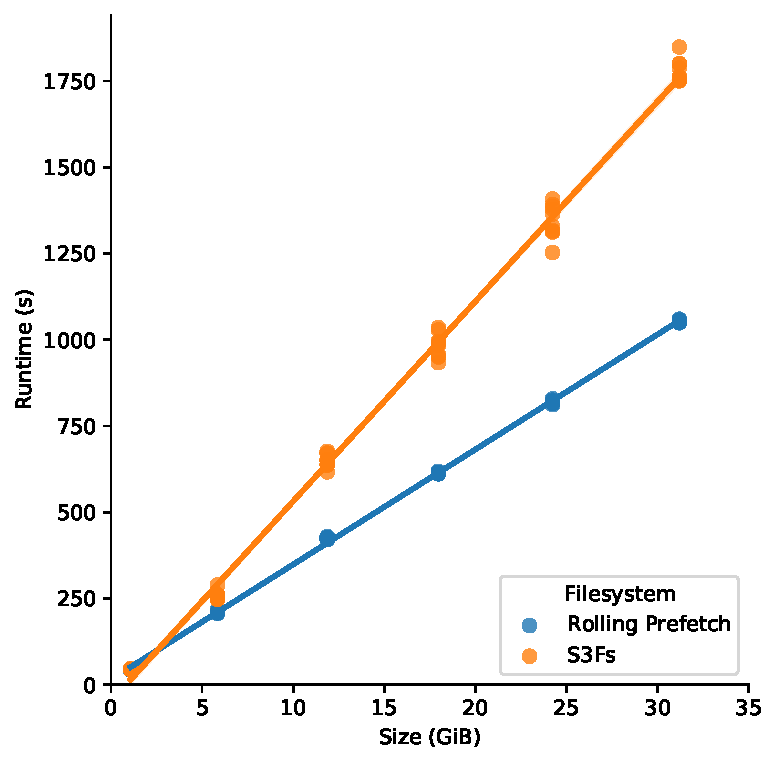
\includegraphics[height=160pt]{figures/rp/filesize.pdf}
%\setlength{\abovecaptionskip}{0pt} \setlength{\belowcaptionskip}{-30pt}
\caption{Runtime performance of reading subsets of the HYDI dataset stored on
Amazon S3 into NiBabel using \sfs and Rolling Prefetch on an Amazon EC2
t2.xlarge instance. Blocksize was set to \SI{64}{\mebi\byte} on both \sfs and
Rolling Prefetch. Prefetch cache consisted of \SI{2}{\gibi\byte} tmpfs storage.}
\label{fig:rp:filesize}
\end{center}
\end{figure}

\begin{figure}
\begin{center}
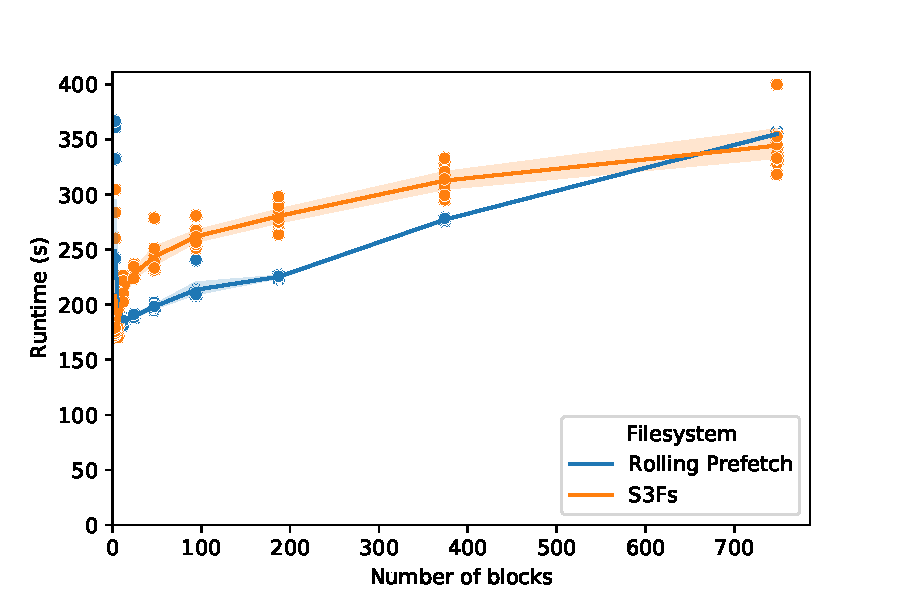
\includegraphics[width=\columnwidth]{figures/rp/blocksize.pdf}
%\setlength{\abovecaptionskip}{-10pt} \setlength{\belowcaptionskip}{-10pt}
\caption{Runtime performance of reading a \SI{6}{\gibi\byte} subset of the HYDI
dataset stored on Amazon S3 into NiBabel using \sfs and Rolling Prefetch with
various block size configurations on an Amazon EC2 t2.xlarge instance. Prefetch
cache consisted of  \SI{2}{\gibi\byte} tmpfs storage.}
%\vspace{-1.5em}
\label{fig:rp:blocksize}
\end{center}
\end{figure}

\begin{figure}
\begin{center}
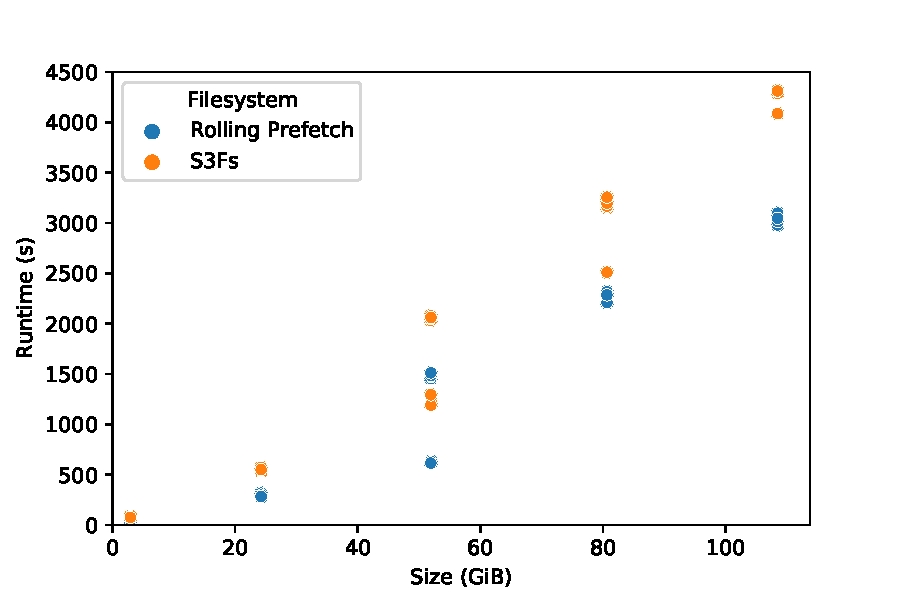
\includegraphics[width=\columnwidth]{figures/rp/parallel.pdf}
%\setlength{\abovecaptionskip}{-10pt} \setlength{\belowcaptionskip}{-20pt}
\caption{Runtime performance of reading subsets of the HYDI dataset stored on
Amazon S3 into NiBabel in parallel using 4 \sfs and Rolling Prefetch processes.
Blocksize was set to \SI{64}{\mebi\byte} on both \sfs and Rolling Prefetch.
Prefetch cache consisted of \SI{1}{\gibi\byte} tmpfs storage.}
%\vspace{-6.5em}
\label{fig:rp:parallel}
\end{center}
\end{figure}



% \begin{figure} \begin{center}
% 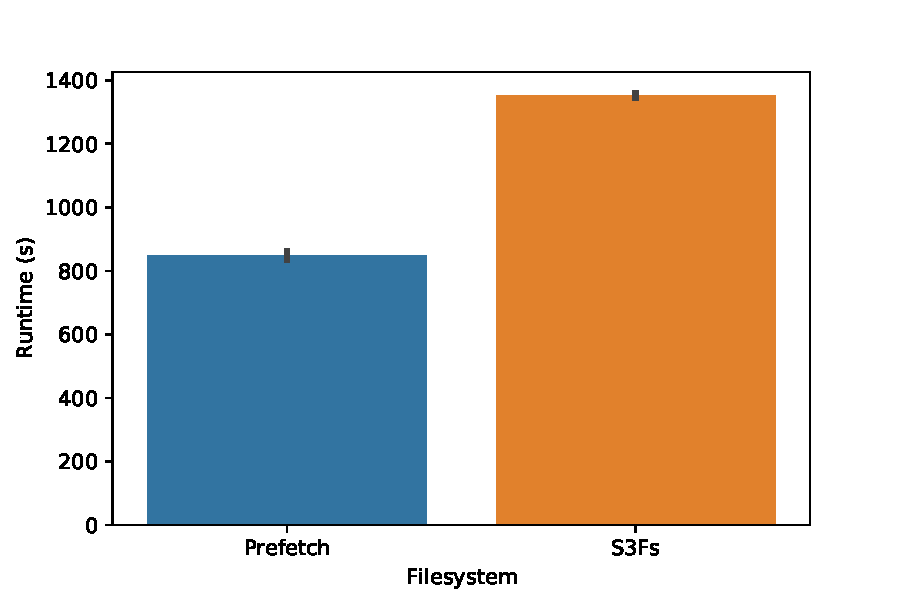
\includegraphics[width=\columnwidth]{figures/segmentation.pdf}
% \caption{Runtime performance of the Segmentation pipeline operating on a
% \SI{1}{\gibi\byte} S3 HYDI tractography file using \sfs and prefetch on an
% Amazon C5.9xlarge instance. Blocksize was set to be \SI{64}{\mebi\byte} on
% both \sfs and prefetch. Prefetch was allotted \SI{2}{\gibi\byte} of storage on
% tmpfs.} \label{fig:segmentation} \end{center} \end{figure}

\begin{figure}
\begin{center}
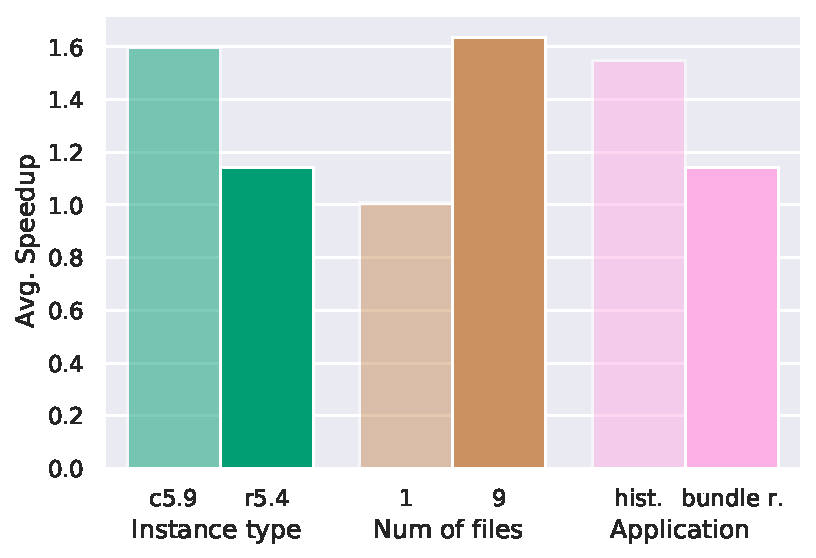
\includegraphics[width=\columnwidth]{figures/rp/speedup.pdf}
%\setlength{\abovecaptionskip}{-10pt} \setlength{\belowcaptionskip}{-8pt}
\caption{Rolling prefetch speedup of the neuroimaging use-cases (histogram and bundle recognition) in various conditions. Experiments varying instance type and number of files were only performed with the bundle recognition pipeline.} 
%\vspace{-1.5em}
\label{fig:rp:speedup}
\end{center}
\end{figure}


\section{Discussion}

Our theoretical analysis and experimental results demonstrate that there is a
substantial processing time gain to be obtained from using Rolling Prefetch,
particularly in the case of mixed workloads, where there is a significant cost
associated with time spent on compute and data transfers. This works well with
typical use cases in neuroimaging, where tasks vary widely ranging from very
short tasks to long ones necessitating hours to complete and where datasets are
large enough to incur transfers of similar magnitudes. Moreover, to save time
with data transfers, researchers may opt to transfer their data over the compute
instance, and perform the computation exclusively with data stored locally.
While this does effectively give the optimal performance during processing,
researchers are left to manage the data themselves. Since local storage on
compute can become quite costly, researchers must decide between processing only
a subset of the data, paying hefty fees related to storing large amounts of data
or incorporating data management logic directly into their workflows. 

There are also natural limitations to Rolling Prefetch. For instance, in the
case of parallel workloads, in certain instances S3 would be preferred to the
available local storage. This is a consequence of the fact that S3 is designed
to be scalable and is capable of processing many requests simultaneously,
whereas unless configured to do so, local storage will not scale adequately to
increased contention.
% Additionally, when blocks become significantly large with an equally large
% number of blocks, it is possible that rolling prefetch will be slower than
% \sfs. -- commented out because cannot remember what i meant 


\subsection{Benefits of Rolling Prefetch}

Rolling Prefetch is an added layer on top of \sfs that replaces its built-in
cache strategies to intercept application read calls and ensure that data is
preloaded. The implementation ensures that file system space requirements are not
exceeded during prefetching through limits set by the user. With the built-in
eviction mechanism, users are not required to do any form of data management
should they be processing datasets larger than available storage. Furthermore,
the library allows configuration of multiple storage device as cache for
prefetching. Currently, files are written to specific storage devices based on
available space and storage priority.

With just a simple data loading workload, we have observed up to a 1.8$\times$
speedup and a maximum overhead of 1.03$\times$. These observed speedups were
obtained when we set the cache location to a \texttt{tmpfs} device and may
naturally decrease with a slower device such as an SSD. In our particular case,
the speedups meant saving 20~min of processing time on loading nearly
\SI{100}{\gibi\byte} of data with a maximum runtime of approximately 71~min.
Moreover, this was achieved on a small instance with only \SI{1}{\gibi\byte} of
prefetch storage allotted to each parallel process, indicating that we can
achieve good speedups even when resources are constrained. 

While our results pertain to the applicability of Rolling Prefetch to
neuroimaging, similar speedups can be expected from other kinds of sequential
processing, such as standard text file processing like word count.

\subsection{Parallelism-related overheads}

While our experiments demonstrate that Rolling Prefetch continues to provide a
performance improvement to parallel applications running on S3, we do expect
performance to decrease if we continue to scale horizontally on a single
instance, or use a slower device as cache. Our implementation consists of two
threads actively reading and writing to local storage. Each time the number of
Rolling Prefetch instances increase, we double the amount of threads writing to
local storage. Although it is standard to have multiple DIMMs on a single
machine, it may not be necessarily true of other storage devices. That being
said, attached cloud volumes may also be sufficiently scalable such that
processing time remains unaffected by an increase in processes.

To reduce the load of prefetching data to local storage, we can add a third
component to Rolling Prefetch that periodically tracks cache bandwidth. Using
such a parameter, the algorithm could take into consideration filesystem load in
addition to user-specified priority.


\subsection{Task granularity}
\sfs was designed to be used within distributed processing frameworks. With such
frameworks, we must take into consideration task granularity and how that would
affect scheduling. Rolling prefetch becomes beneficial with larger files.
Assuming a workload where the task is simply to load the streamlines, we would
need a few GBs of data to start noticing a speedup. In cases where resources are
ample enough to run all tasks in parallel and the amount of data processed by a
task is minimal, Rolling Prefetch and \sfs would probably behave similarly, with
\sfs potentially performing a bit faster.

The risk with passing large amounts data to the library within a task is that it
is less robust to failures as any failed task would have to resume from the
beginning. This could take a significant amount of time, depending on how much
data had been processed by the task prior to failure.
% Making the tasks smaller would reduce the costs associated with task restart,
% but then the benefits of Rolling Prefetch would be limited.
It is understandable that implementations such as Netco are adaptations to
persistent file system, since then prefetching could work without limiting
scheduler logic. For our implementation to be efficient within parallel
processing frameworks, we would need to decouple it from the task itself and
allow it to communicate with the task scheduler to determine which files to
prefetch.



\section{Conclusion}

% Prefetching is a widely used method for minimizing the costs of computational
% workloads that involve multiple data reads. To determine the potential added
% value of prefetching to large-scale neuroimaging workloads, we quantified its
% speedup through analysis of the runtime performance of standard neuroscience
% data loading, and by embedding this idea in existing computational pipelines.
% To accomplish this, we developed Rolling Prefetch, a Python library that can
% prefetch sequentially-read binary files located on S3 as an extension of the
% \sfs library. We compared the performance of Rolling Prefetch with \sfs. While
% there have been implementations for prefetching on the cloud, this technique
% has not been used for the processing of neuroscience workloads on the cloud.
% However, this idea is becoming more relevant for neuroscience data analysis
% workloads, as contemporary neuroscience datasets continue to increase in size
% and analysis pipelines are becoming more data-intensive.

% Our theoretical analysis of prefetching concluded that Rolling Prefetch can
% provide up to a maximum of 2x speedup, and is most effective when the time
% needed to compute is comparable to the time required to transfer the data.
% Furthermore, it was determined that while \sfs performed best given the least
% number of blocks, Rolling Prefetch would perform best with an intermediary
% number of blocks, where the overheads of prefetching would become more
% significant at 1 block, when prefetching would at minimum do the same amount
% of work as \sfs, and at many blocks, where the latency of writing locally
% would become apparent. Overall the analysis states that it is better to
% slightly overestimate the number of blocks as the penalty of reading more
% blocks is proportional to the latency of the cloud ($l_{c}$).

% Our experimental evaluation supports the conclusions drawn from the
% theoretical evaluation. A peak speedup of 1.8x was attained when processing a
% total of 20 tractography files across four parallel threads. Good speedups
% were also obtained when increasing the number of files processed per task,
% obtaining a 1.7x speedup at 25 files. As determined by our theoretical
% evaluation, having too few blocks and too many blocks penalized the
% performance of Rolling Prefetch due to overheads incurred by the prefetching
% process.

Overall, we conclude that Rolling Prefetch would be a valuable addition to
large-scale neuroimaging pipelines executing on the cloud, particularly in
instances where data transfer and compute time are similar. 
% However, our implementation still has limitations that may not make it
% favorable to distributed processing. 
Future work should focus on the following improvements: The loading part of
Rolling Prefetch should be performed outside of task themselves to ensure that
it does not interrupt any form of task scheduling and to avoid tasks which take
too long to restart if lost. The library should also communicate with schedulers
to help determine where tasks should be scheduled given the location of the
data.
